\subsection{Algoritmo ottimizza debiti}

\subsubsection{PseudoCodice}
\begin{figure}[H]
    \centering
    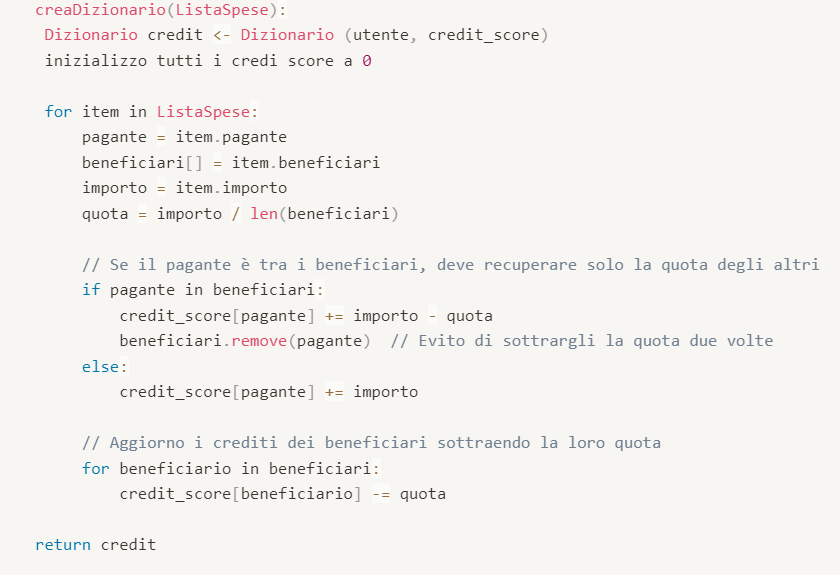
\includegraphics[scale=0.8]{images/CreaDizionario.png}
    \caption{Funzione CreaDizionario}
\end{figure}

\begin{figure}[H]
    \centering
    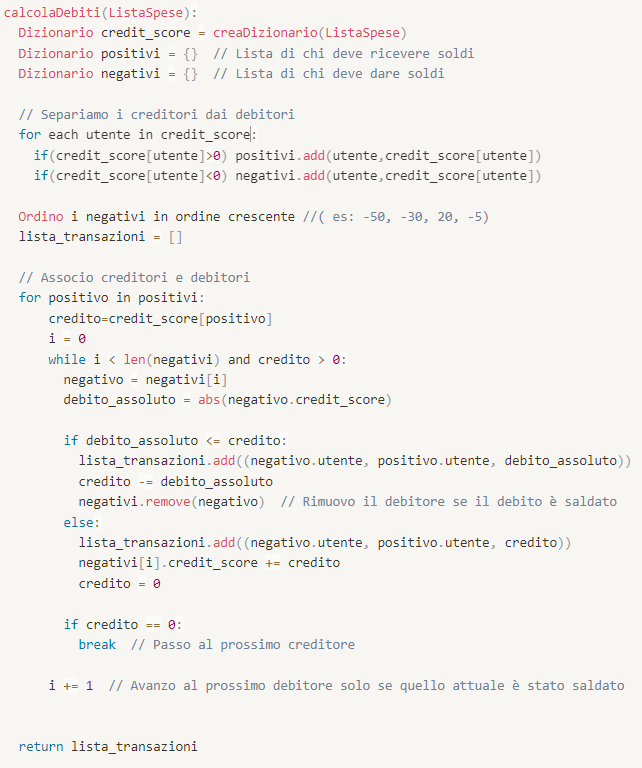
\includegraphics[scale=0.8]{images/CalcolaDebiti.png}
    \caption{Funzione CalcolaDebiti}
\end{figure}


\subsubsection{Descrizione}

La funzione \texttt{CreaDizionario} prende in input una matrice di spese e costruisce un dizionario in cui:

\begin{itemize}
    \item La chiave è lo \textit{username} dell’utente.
    \item Il valore è il suo \textit{credit score}, che indica quanto deve ricevere o restituire.
\end{itemize}

Scorrendo i record della matrice, la funzione aggiorna progressivamente i \textit{credit score} degli utenti.


Se il \textit{credit score} è positivo, l’utente deve ricevere soldi.
Se invece è negativo, deve restituire una somma.


La funzione \texttt{calcolaDebiti} utilizza \texttt{CreaDizionario} per ottenere il saldo di ogni utente.
A questo punto, suddivide gli utenti in due liste:

\begin{itemize}
    \item \textbf{Creditori}: utenti con \textit{credit score} positivo.
    \item \textbf{Debitori}: utenti con \textit{credit score} negativo, ordinati in modo crescente.
\end{itemize}

Per ogni creditore, si scorre l’elenco dei debitori per saldare i crediti:

\begin{enumerate}
    \item Se il debito di un utente è minore o uguale al credito disponibile:
    \begin{itemize}
        \item Si sottrae l’intero importo dal credito.
        \item La transazione viene registrata.
        \item Il debitore viene rimosso dalla lista, poiché ha estinto il suo debito.
        \item Se il credito arriva a zero, si interrompe l’iterazione e si passa al creditore successivo.
    \end{itemize}
    \item Se invece il debito è maggiore del credito:
    \begin{itemize}
        \item Si utilizza tutto il credito disponibile per ridurre il debito.
        \item La transazione viene registrata.
        \item Il debitore rimane nella lista, poiché ha ancora un saldo negativo da coprire.
        \item Il credito diventa zero e si passa al creditore successivo.
    \end{itemize}
\end{enumerate}


\subsubsection{Complessità}

La funzione \texttt{CreaDizionario} ha:

\begin{itemize}
    \item Un ciclo esterno che itera su tutti gli elementi della matrice $\rightarrow O(n)$
    \item Un ciclo interno che itera su tutti i beneficiari di ogni record $\rightarrow O(n)$
\end{itemize}

Essendo i due cicli annidati, la complessità totale è: $O(n^2)$.

La funzione \texttt{CalcolaDebiti} esegue le seguenti operazioni:

\begin{enumerate}
    \item Richiama \texttt{CreaDizionario} $\rightarrow O(n^2)$
    \item Itera sul dizionario per separare creditori e debitori $\rightarrow O(n)$
    \item Ordina la lista dei debitori  $\rightarrow O(n \log n)$
    \item Associa creditori e debitori
    \begin{itemize}
        \item Itera su tutti i creditori $\rightarrow O(n)$
        \item Per ogni creditore, nel caso peggiore, può iterare su tutti i debitori $\rightarrow O(n)$
        \item Complessità totale del ciclo annidato $\rightarrow O(n^2)$
    \end{itemize}
\end{enumerate}

Sommiamo i contributi principali:

\[ O(n^2) + O(n) + O(n \log n) + O(n^2) = O(n^2) \]

Complessità finale: $O(n^2)$